\chapter{Methodology}
\label{ch:methodology}

This chapter sets out the research approach, the threat model, the target topology, and the formal definitions of the metrics used to evaluate it. The intention is that any reader with the source code in Appendix~\ref{ch:appendix-dockerfiles}--\ref{ch:appendix-helper} should be able to reproduce the experiments, obtain comparable numerical outputs, and challenge the conclusions on the basis of the same evidence.

\section{Research Approach}

The work follows a \emph{controlled comparative experiment} design. Two systems --- the flat (control) and segmented (treatment) topologies --- are constructed so that they are identical in every respect except for the variable under study, namely whether internal traffic is filtered. The same workloads are applied to each, and the same measurements are taken. This design is consistent with the empirical methodology recommended for security research by \textcite{Sommer and Paxson}{2010}, who emphasise the importance of explicit baselines, reproducibility, and the isolation of the variable under test.

The independent variable is the network architecture (\emph{flat} or \emph{segmented}), encoded in the Docker Compose configuration and the firewall rule set. The dependent variables are the four metrics defined in Section~\ref{sec:metrics}. All other parameters --- the host operating system, the container image, the number and identity of internal hosts, the services they expose, the test sequence, and the number of iterations --- are held constant.

\section{Threat Model}
\label{sec:threat-model}

Following the structured threat-modelling approach recommended by \textcite{Howard and LeBlanc}{2003}, the threat model is stated explicitly in terms of assets, adversaries, capabilities, and assumptions.

\paragraph{Assets} The assets of interest are (i) a public-facing web server, (ii) an internal file server (SMB), (iii) an internal database (MySQL), (iv) administrative workstations, and (v) the user data implicitly held on student and staff endpoints.

\paragraph{Adversaries} Two adversarial roles are modelled. The \emph{external attacker} is located on a separate \texttt{external} subnet (\texttt{192.168.100.0/24} for flat, \texttt{192.168.200.0/24} for segmented) and represents the Internet. The \emph{internal attacker} is a compromised student workstation that has obtained foothold via, for example, a phishing email --- the most common initial-access vector in modern intrusions according to \textcite{Verizon}{2023}.

\paragraph{Capabilities} Both adversaries are assumed to possess the standard tools available in any modern Linux distribution: \texttt{ping}, \texttt{nc}, \texttt{nmap}, and \texttt{curl}. They cannot escape the container; they cannot exploit the firewall itself; they do not possess credentials for any internal service. They are assumed to be capable of network reconnaissance and of attempting to connect to any host they can route to.

\paragraph{Assumptions} The firewall enforces only network-layer policy. Application-layer authentication, encryption, and host-based intrusion detection are out of scope. The host operating system is trusted. These simplifications are consistent with the scope of the project (see Section~1.4) and are revisited in the limitations discussion in Chapter~\ref{ch:discussion}.

\paragraph{Mapping to MITRE ATT\&CK} The model exercises the following techniques from \textcite{MITRE}{2024}: T1018 (\textit{Remote System Discovery}), T1046 (\textit{Network Service Scanning}), and T1021 (\textit{Remote Services}). Segmentation, when applied, prevents the latter two techniques in respect of any host that lies in a different zone from the attacker.

\section{Reference Topology}
\label{sec:topology}

The reference topology, illustrated in Figure~\ref{fig:topo-flat} and Figure~\ref{fig:topo-segmented}, models a small campus environment with ten participants in two configurations.

\begin{figure}[H]
\centering
\begin{tikzpicture}[
    every node/.style={font=\small},
    host/.style={draw, rounded corners=2pt, minimum width=1.6cm, minimum height=0.7cm, fill=blue!5},
    fw/.style={draw, rounded corners=2pt, minimum width=2.0cm, minimum height=0.8cm, fill=red!10},
    attacker/.style={draw, rounded corners=2pt, minimum width=2.0cm, minimum height=0.8cm, fill=orange!20},
    cloud/.style={draw, ellipse, fill=gray!10, minimum width=4cm, minimum height=1.4cm},
    line/.style={-, thick, gray!70}
]
\node[attacker] (att) at (-4.2,2.3) {attacker};
\node[fw] (fw) at (0,2.3) {firewall};
\node[cloud] (lan) at (0,0) {flat\_internal\;\;\;10.10.0.0/24};
\node[host] (s1) at (-5.0,-1.6) {student};
\node[host] (s2) at (-3.5,-1.6) {student2};
\node[host] (st) at (-2.0,-1.6) {staff};
\node[host] (ad) at (-0.5,-1.6) {admin};
\node[host] (we) at (1.0,-1.6) {web};
\node[host] (fi) at (2.5,-1.6) {file};
\node[host] (db) at (4.0,-1.6) {db};
\node[host] (io) at (-3.0,-2.6) {iot};
\node[host] (gu) at (-1.5,-2.6) {guest};
\draw[line] (att) -- (fw);
\draw[line] (fw) -- (lan);
\draw[line] (lan.south) -- (s1.north);
\draw[line] (lan.south) -- (s2.north);
\draw[line] (lan.south) -- (st.north);
\draw[line] (lan.south) -- (ad.north);
\draw[line] (lan.south) -- (we.north);
\draw[line] (lan.south) -- (fi.north);
\draw[line] (lan.south) -- (db.north);
\draw[line] (lan.south) -- (io.north);
\draw[line] (lan.south) -- (gu.north);
\end{tikzpicture}
\caption[Flat topology]{Flat topology: all internal hosts share a single \texttt{/24} subnet behind a single perimeter firewall.}
\label{fig:topo-flat}
\end{figure}

\begin{figure}[H]
\centering
\begin{tikzpicture}[
    every node/.style={font=\footnotesize},
    host/.style={draw, rounded corners=2pt, minimum width=1.4cm, minimum height=0.6cm, fill=blue!5},
    fw/.style={draw, rounded corners=2pt, minimum width=2.0cm, minimum height=0.8cm, fill=red!10},
    attacker/.style={draw, rounded corners=2pt, minimum width=2.0cm, minimum height=0.8cm, fill=orange!20},
    zone/.style={draw, dashed, rounded corners=4pt, fill=gray!7, inner sep=4pt},
    line/.style={-, thick, gray!70}
]
\node[attacker] (att) at (0,4) {attacker};
\node[fw] (fw) at (0,2.5) {gateway firewall};
\draw[line] (att) -- (fw);

\node[host] (s1) at (-6,0.5) {student};
\node[host] (s2) at (-4.5,0.5) {student2};
\begin{scope}[on background layer]
\node[zone, fit=(s1)(s2), label=above:{\textbf{student\_net}}] {};
\end{scope}

\node[host] (st) at (-2.5,0.5) {staff};
\begin{scope}[on background layer]
\node[zone, fit=(st), label=above:{\textbf{staff\_net}}] {};
\end{scope}

\node[host] (ad) at (-0.6,0.5) {admin};
\begin{scope}[on background layer]
\node[zone, fit=(ad), label=above:{\textbf{admin\_net}}] {};
\end{scope}

\node[host] (we) at (1.5,0.5) {web};
\node[host] (fi) at (3.0,0.5) {file};
\node[host] (db) at (4.5,0.5) {db};
\begin{scope}[on background layer]
\node[zone, fit=(we)(fi)(db), label=above:{\textbf{server\_net}}] {};
\end{scope}

\node[host] (io) at (-2.5,-1.5) {iot};
\begin{scope}[on background layer]
\node[zone, fit=(io), label=below:{\textbf{iot\_net}}] {};
\end{scope}

\node[host] (gu) at (1.5,-1.5) {guest};
\begin{scope}[on background layer]
\node[zone, fit=(gu), label=below:{\textbf{guest\_net}}] {};
\end{scope}

\foreach \n in {s1,s2,st,ad,we,fi,db,io,gu}{
    \draw[line] (fw) -- (\n);
}
\end{tikzpicture}
\caption[Segmented topology]{Segmented topology: six independent \texttt{/24} subnets, all routed through a single firewall enforcing zone-to-zone policy.}
\label{fig:topo-segmented}
\end{figure}

Figure~\ref{fig:screenshot-flat} and Figure~\ref{fig:screenshot-segmented} show the Docker Compose environments as observed in the running testbed, confirming that the container names, IP addresses, and network attachments match the design above.

\begin{figure}[H]
\centering
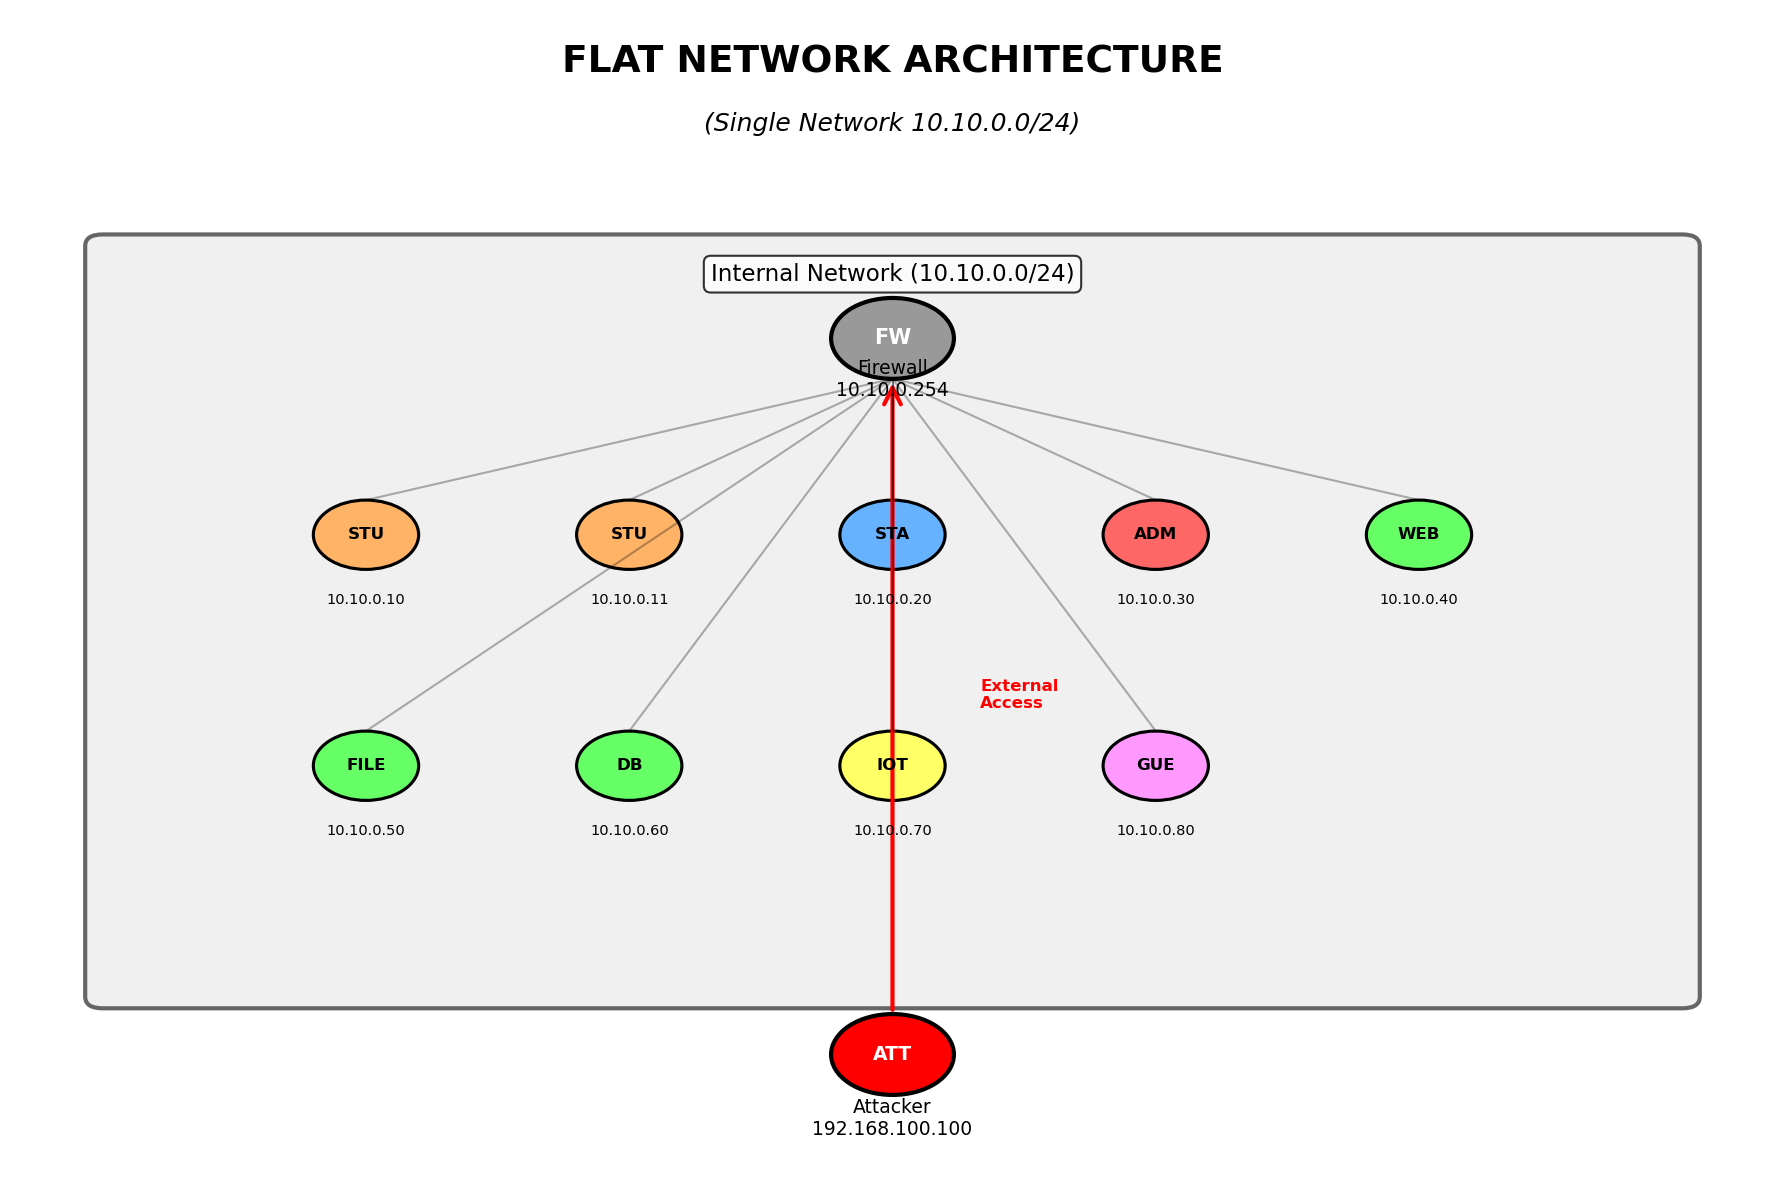
\includegraphics[width=0.90\textwidth]{figures/flat_network.png}
\caption[Flat topology --- running testbed]{Running flat topology in Docker: all ten containers attached to a single \texttt{flat\_internal} bridge network (\texttt{10.10.0.0/24}).}
\label{fig:screenshot-flat}
\end{figure}

\begin{figure}[H]
\centering
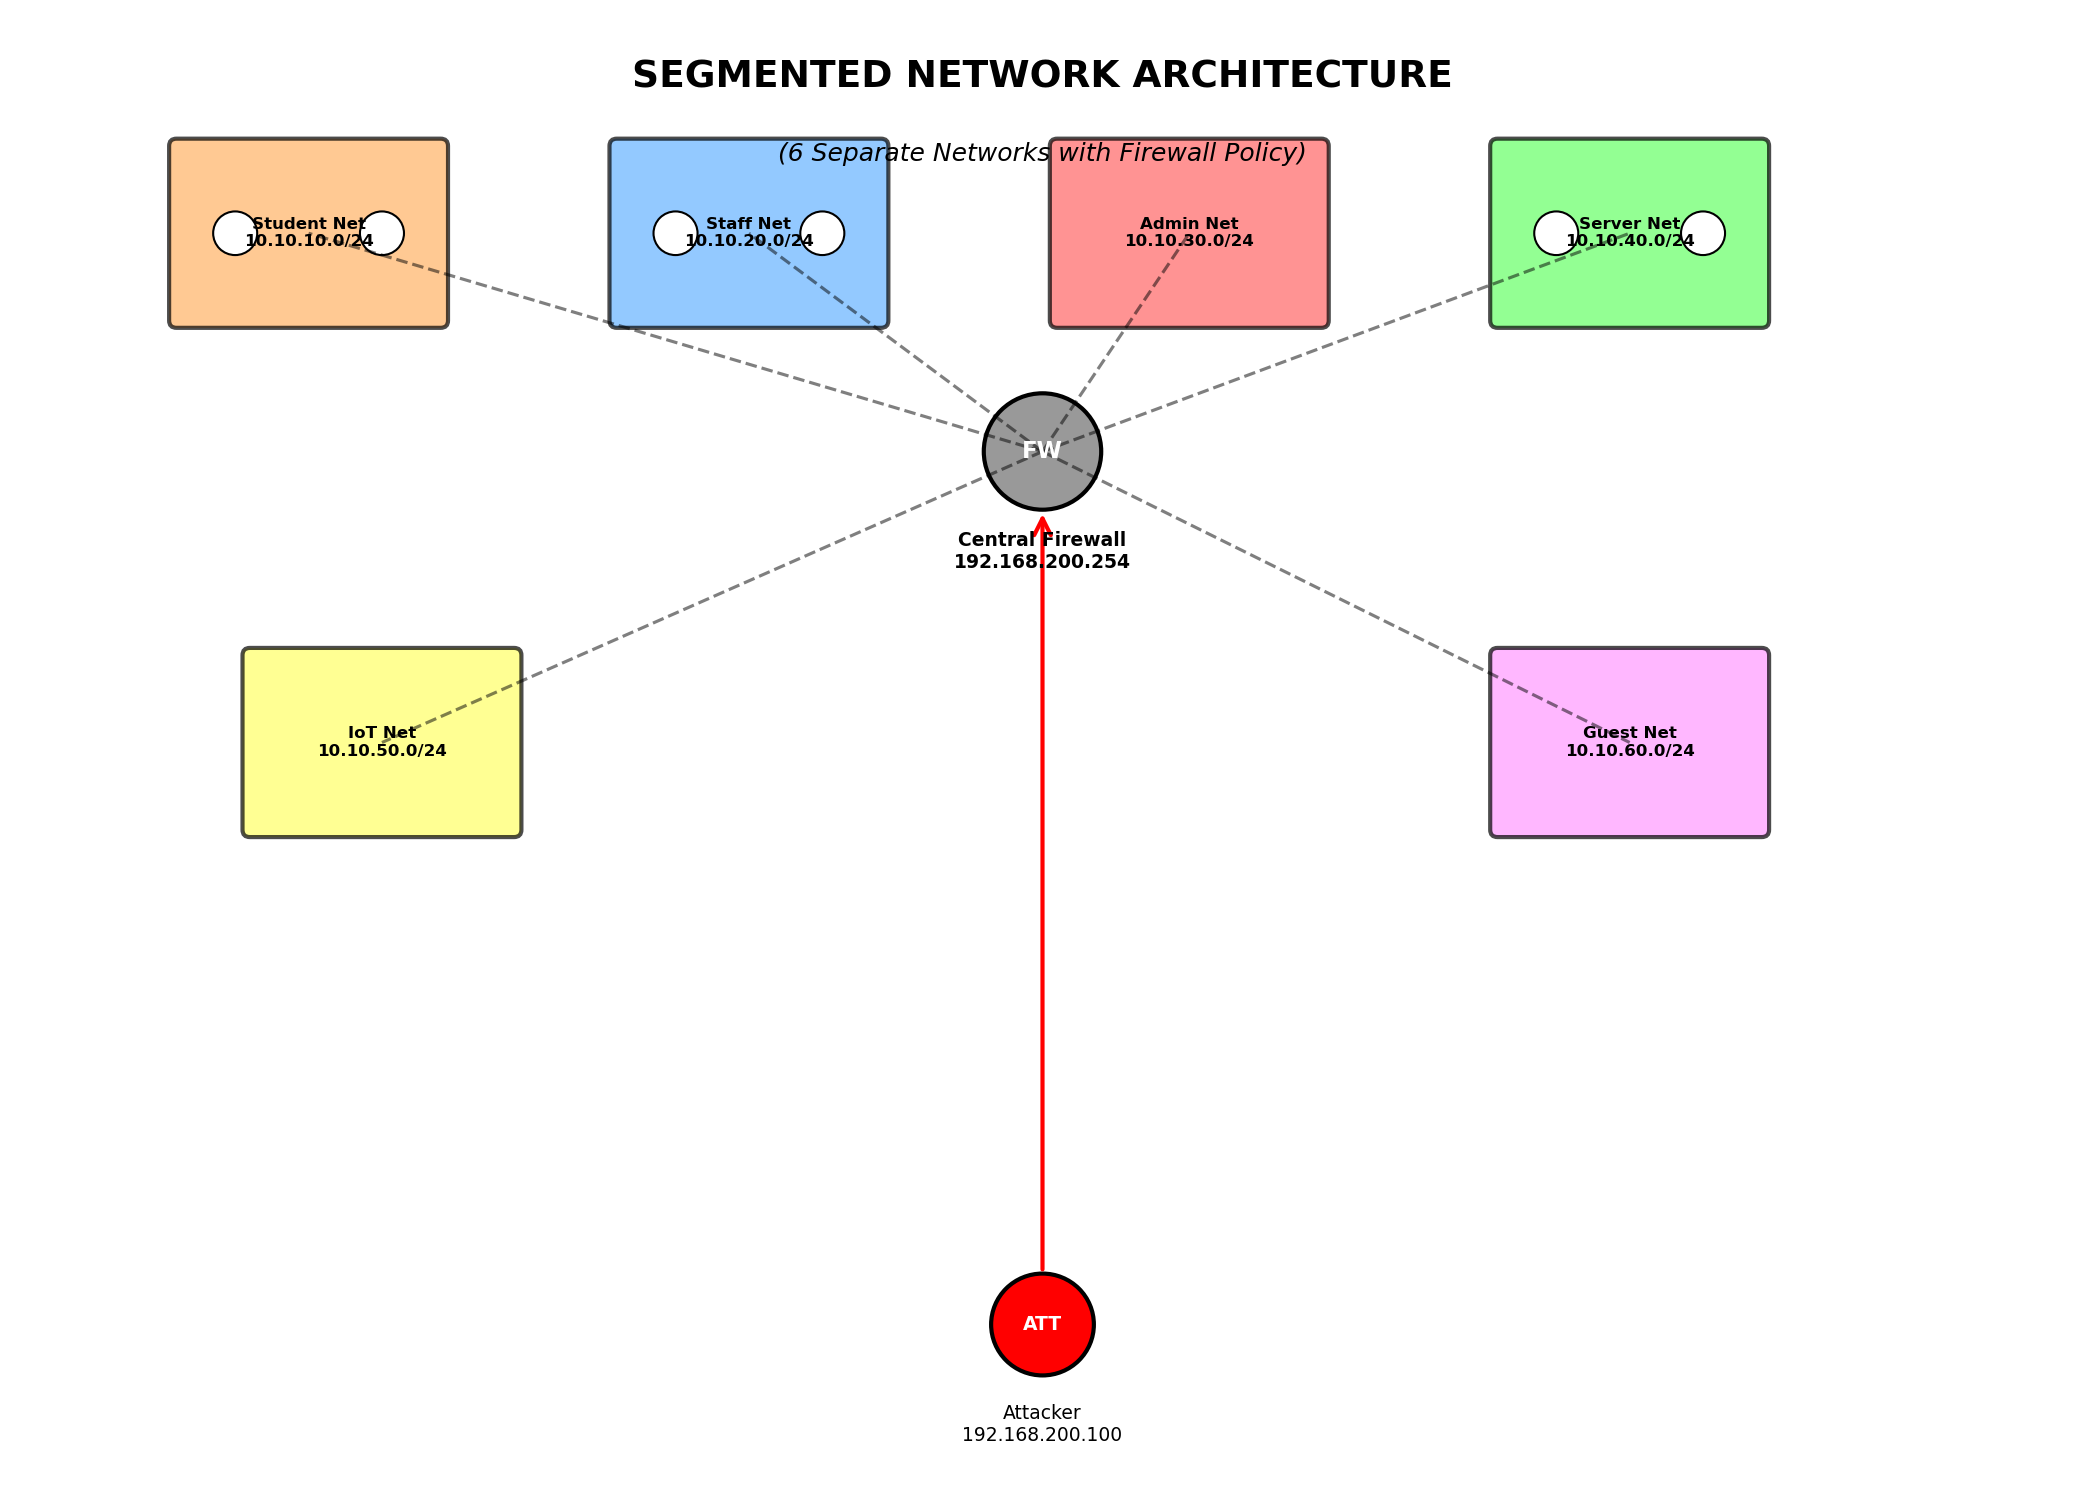
\includegraphics[width=0.90\textwidth]{figures/segmented_network.png}
\caption[Segmented topology --- running testbed]{Running segmented topology in Docker: each host is attached to exactly one zone network, with the gateway container bridging all six zones.}
\label{fig:screenshot-segmented}
\end{figure}

The flat topology places all ten hosts in a single \texttt{/24} subnet (\texttt{10.10.0.0/24}). The perimeter firewall protects this subnet from the external attacker but does not filter internal traffic. The segmented topology decomposes the same set of hosts into six purpose-defined zones --- \texttt{student\_net}, \texttt{staff\_net}, \texttt{admin\_net}, \texttt{server\_net}, \texttt{iot\_net}, \texttt{guest\_net} --- each implemented as a separate Docker network with its own \texttt{/24} subnet. A single gateway firewall has interfaces on all six zones plus the external network and enforces a default-deny policy with explicit allow rules for legitimate flows.

The choice of six zones reflects the categories most commonly recommended in segmentation guidance \parencite{NCSC}{2018}; \parencite{CIS}{2024}: untrusted users (students, guests), trusted users (staff), privileged users (administrators), production servers, untrusted devices (IoT), and the external boundary. The zones are deliberately functional rather than departmental, in line with the principle of role-based segmentation \parencite{Hu et al.}{2014}.

\section{Evaluation Metrics}
\label{sec:metrics}

Four primary metrics and one composite metric are computed. The definitions below are stated formally so that they can be replicated and compared with future work.

\subsection{Firewall Policy Accuracy}

Let $T$ denote the set of connectivity tests, each of which specifies a source host, a destination host, a port, and an expected outcome ($\textsc{allow}$ or $\textsc{block}$). For each test $t \in T$ the harness records the observed outcome $o_t$ and the expected outcome $e_t$. Policy accuracy is defined as

\begin{equation}
A_{\textit{policy}} \;=\; \frac{|\{t \in T : o_t = e_t\}|}{|T|} \times 100\%.
\label{eq:accuracy}
\end{equation}

This metric formalises the property identified by \textcite{Wool}{2004} as the most important predictor of effective firewall deployment: that the rules actually do what their author intended.

\subsection{Blast-Radius Exposure}

Let $H$ denote the set of internal target hosts other than the compromised foothold, and for each host $h \in H$ define the indicator $r_h = 1$ if $h$ is reachable from the foothold over the relevant port (TCP/80, TCP/445, TCP/3306, or ICMP, as appropriate to the service offered), and $0$ otherwise. The blast-radius exposure is

\begin{equation}
B \;=\; \frac{1}{|H|}\sum_{h \in H} r_h \times 100\%,
\label{eq:blast}
\end{equation}

with the corresponding \emph{containment score} defined as $C = 100\% - B$. Lower blast-radius is better; higher containment is better. This formulation matches the definition used in NIST SP~800-207 \parencite{Rose et al.}{2020} and is the metric most directly meaningful to security practitioners.

\subsection{Performance Metrics}

A volume of HTTP requests is issued from a non-administrator client (the student workstation) to the public web server. Two metrics are derived from the resulting log of $N = 500$ requests per scenario:

\begin{itemize}[leftmargin=*]
    \item \textbf{Availability} $\textsc{Av} = \frac{|\{i : code_i = 200\}|}{N} \times 100\%$, the proportion of requests that returned an HTTP 200 status.
    \item \textbf{Average response time} $\overline{t} = \frac{1}{N_{200}}\sum_{i: code_i=200} t_i$, the mean elapsed time over successful requests.
\end{itemize}

These follow standard practice in network performance benchmarking and are consistent with the definitions used by \textcite{Stallings}{2020}.

\subsection{Composite Reliability Index}

A single weighted-sum composite metric is computed for each scenario as

\begin{equation}
R \;=\; 0.30\,\textsc{Av} \;+\; 0.35\,C \;+\; 0.25\,A_{\textit{policy}} \;+\; 0.10\,P,
\label{eq:reliability}
\end{equation}

where $P = \max(0, 100 - 1000\overline{t})$ is a performance score that penalises higher latency. The weights reflect the relative importance assigned to each dimension in the project's brief: availability and containment dominate (combined weight 0.65), policy correctness contributes substantially (0.25), and raw performance is included as a smaller penalty (0.10). The choice is intentionally transparent and follows the weighted-sum approach recommended for security composite indices by \textcite{Cherdantseva and Hilton}{2013}.

\section{Test Procedure}

The full test procedure for each scenario is:

\begin{enumerate}[label=\arabic*., leftmargin=*]
    \item Launch the appropriate Docker Compose file and wait for all containers to enter the \texttt{healthy} state.
    \item Apply the corresponding firewall rule set on the gateway container.
    \item Run the \texttt{connectivity\_test.sh} harness, producing a CSV record of expected and observed outcomes.
    \item Run the \texttt{blast\_radius\_test.sh} harness, probing all eight peer hosts from the compromised student workstation.
    \item Run the \texttt{performance\_test.sh} harness, issuing 500 HTTP requests from each of four sources (student, staff, admin, guest).
    \item Run the \texttt{scan\_test.sh} harness from the student container, recording the visible attack surface using Nmap.
    \item Run the \texttt{summarise\_results.py} script to compute all metrics and write \texttt{summary.csv}.
    \item Run the \texttt{make\_plots.py} script to produce all figures used in Chapter~\ref{ch:results}.
\end{enumerate}

The same script set is used for both scenarios; only the scenario name is different. The full source listing is reproduced in Appendix~\ref{ch:appendix-tests}.

\section{Reproducibility}

In keeping with the recommendations of \textcite{Sommer and Paxson}{2010}, every component of the experiment is captured in declarative source files: a single Dockerfile, two Docker Compose files, two firewall scripts, and a small set of test scripts. The container image is pinned by tag (\texttt{handsonsecurity/seed-ubuntu:large}). The experiment can be executed end-to-end on any host with Docker Engine 20.10 or later and at least 4~GB of free RAM. The total execution time for both scenarios is approximately 18~minutes. All raw data and figures presented in Chapter~\ref{ch:results} are derived by these scripts and can therefore be regenerated on demand.
